\documentclass[20pt, a4paper]{article}
\usepackage[urlcolor=blue, colorlinks, linkcolor=blue]{hyperref}
\usepackage{graphicx}
\usepackage{subfig}


\begin{document}
\title{Báo cáo đồ án cuối kỳ \\
Máy học thống kê\\
Yolo Object Detection}
\author{1712495 - Nguyễn Quang Huy}
\maketitle

\renewcommand{\abstractname}{Tóm tắt}
\begin{abstract}
	Xây dựng website cho phép người dùng sử dụng mô hình Yolov4-Tiny để nhận dạng đối tượng thường ngày 
	hoặc mô hình đã được điều chỉnh để nhận dạng 5 loài động vật: báo(cheetah), tinh tinh(chimpanzee), sư tử(lion), hươu vàng(hog deer), gấu chó(sun bear). 
\end{abstract}

\renewcommand{\contentsname}{Mục lục}
\tableofcontents

\section{Mô hình Yolov4-Tiny}

\href{https://github.com/AlexeyAB/darknet#pre-trained-models}{Yolov4-Tiny} 
là mô hình nhận dạng đối tượng được huấn luyện trên tập dữ liệu MS COCO với kết quả 40.2\% mAP@0.5.

Để sử dụng mô hình, ta build framework \href{https://github.com/AlexeyAB/darknet}{darknet} và dùng nó cùng với trọng số của mô hình đã được huấn luyện để dự đoán đối tượng trong ảnh bất kỳ

\section{Mô hình nhận dạng động vật}
\subsection{Giới thiệu}
Mô hình này là Yolov4-Tiny được huấn luyện tiếp để nhận dạng 5 loài động vật: báo, tinh tinh, sư tử, hươu vàng, gấu chó.
\subsection{Tập dữ liệu}
\begin{itemize}
	\item
Tập dữ liệu gồm 2093 hình ảnh của 5 loài động vật, được tải về từ chức năng tìm kiếm hình ảnh của Google.\\
Tham khảo các bước cụ thể trong quy trình thu thập dữ liệu tại đây: \href{https://www.pyimagesearch.com/2017/12/04/how-to-create-a-deep-learning-dataset-using-google-images/}{How to create a deep learning dataset using Google Images}

\begin{tabular}{l | r}
	\textbf{Loài} & \textbf{Số hình ảnh} \\
	\hline
	Báo & 538 \\
	Tinh tinh & 561 \\
	Sư tử & 338 \\
	Hươu vàng & 377 \\
	Gấu chó & 279 \\
\end{tabular}

\item
Sau đó dữ liệu được dán nhãn thủ công theo format của Yolo

\item
Cuối cùng, dữ liệu được chia thành 3 tập train, validation, test bằng 
\href{https://scikit-learn.org/stable/modules/generated/sklearn.model\_selection.train\_test_split.html}{sklearn.model\_selection.train\_test\_split} với tỉ lệ lần lượt 75\%, 15\%, 10\%
\end{itemize}

\subsection{Huấn luyện}
\subsubsection{Cách thực hiện}
Để huấn luyện tiếp(fine tuning) mô hình Yolov4-Tiny có sẵn, ta làm theo 
\href{https://github.com/AlexeyAB/darknet#how-to-train-tiny-yolo-to-detect-your-custom-objects}{hướng dẫn của framework darknet}

Cụ thể:
\begin{itemize}
	\item Sử dụng Google Colab
	\item Chọn batch và subdivisions phù hợp với cấu hình máy tính
	\item Chọn max\_batch tùy theo số loại đối tượng(class). Đây chính là số epoch. \\
		Darknet khuyến cáo max\_batch = max(classes*2000, 6000, number of training images)
	\item Chọn network size: width và height. Các ảnh input sẽ được resize về kích thước này
\end{itemize}

\subsubsection{Kết quả}
\begin{enumerate}
	\item Huấn luyện 2 mô hình có network size khác nhau: (width=544, height=544) và (width=640, 640). Số max\_batch đều là 10000 theo công thức của darknet
	\item Sau 10000 max\_batch, kết quả của cả 2 mô hình trên tập validation: 
		\subitem (width=544, height=544): 58.31\% mAP@0.5
		\subitem (width=640, height=640): 49.51\% mAP@0.5
	\item Thử tiếp tục huấn luận thêm 5000 max\_batch nữa thì đạt được kết quả: 
		\subitem (width=544, height=544): 81.58\% mAP@0.5
		\subitem (width=640, height=640): 74.05\% mAP@0.5

		và không có dấu hiệu tăng thêm. 
		
\begin{figure}[h!]
	\centering
	\subfloat[\centering 10000 max\_batch đầu]{{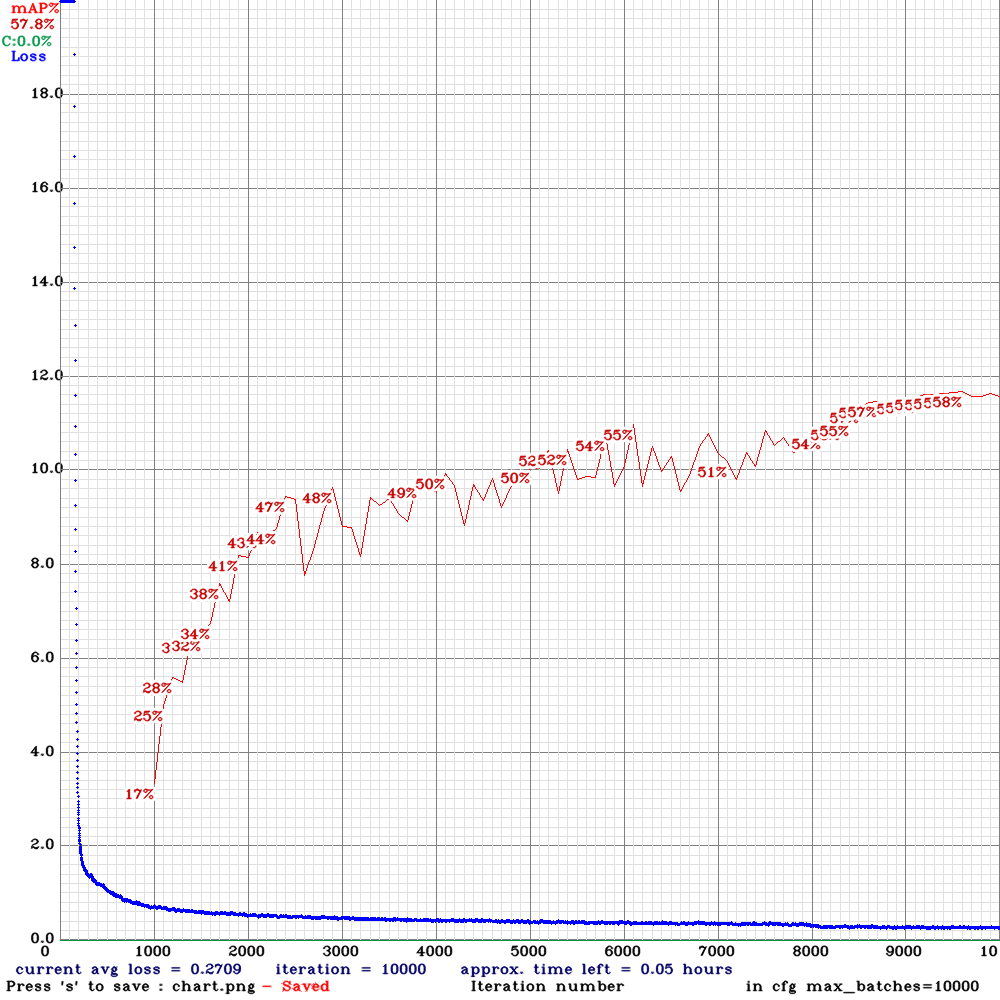
\includegraphics[width=5cm]{544-544-10000/chart.png}}}
	\qquad
	\subfloat[\centering 5000 max\_batch sau]{{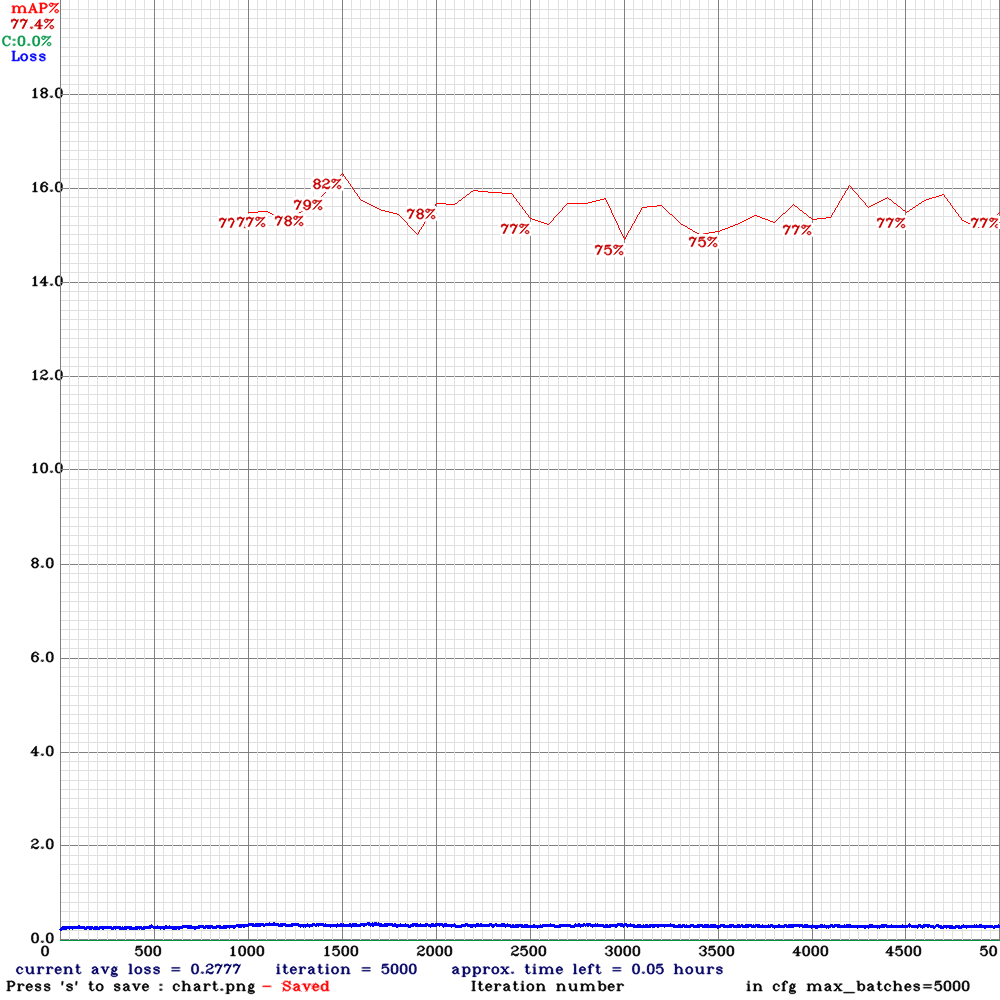
\includegraphics[width=5cm]{544-544-15000/chart.png}}}
	\caption \nolinebreak width=544, height=544 \\ red line: mAP
\end{figure}	
\begin{figure}[h!]
	\centering
\subfloat[\centering 10000 max\_batch đầu]{{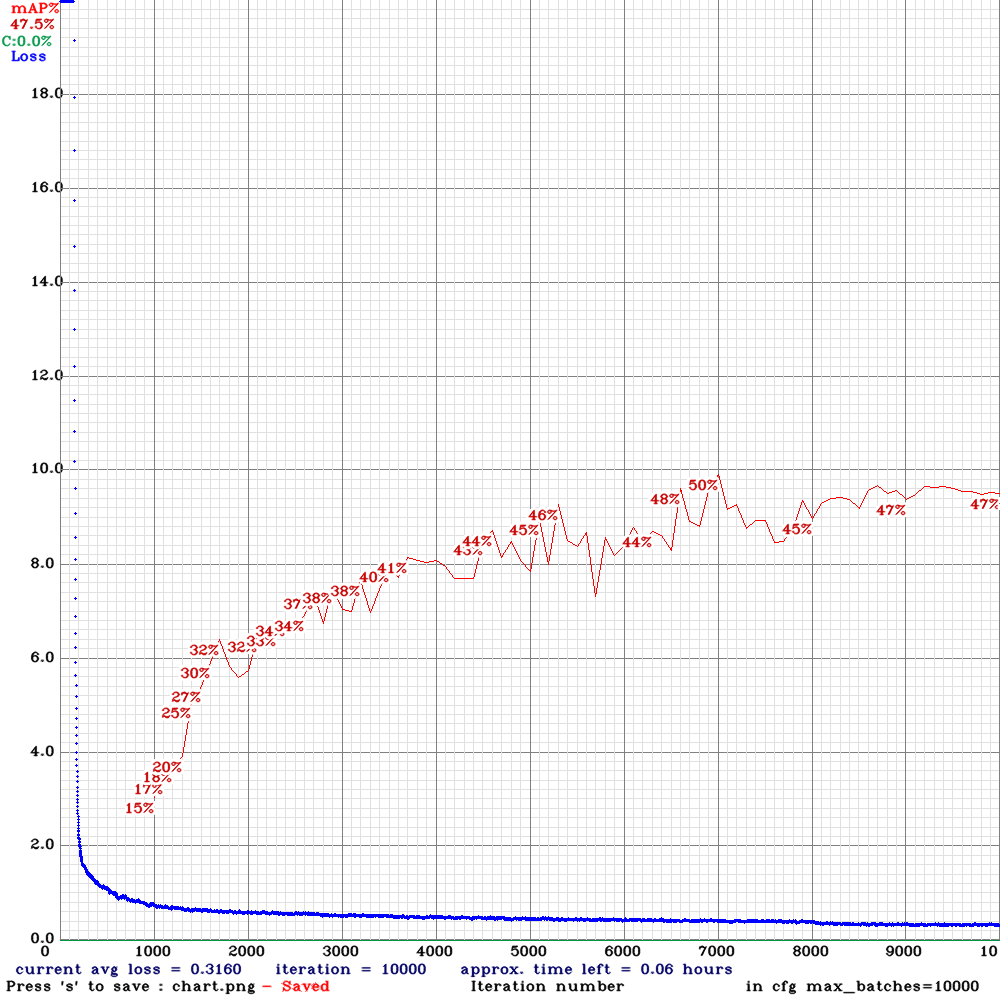
\includegraphics[width=5cm]{640-640-10000/chart.png}}}
	\qquad
	\subfloat[\centering 5000 max\_batch sau]{{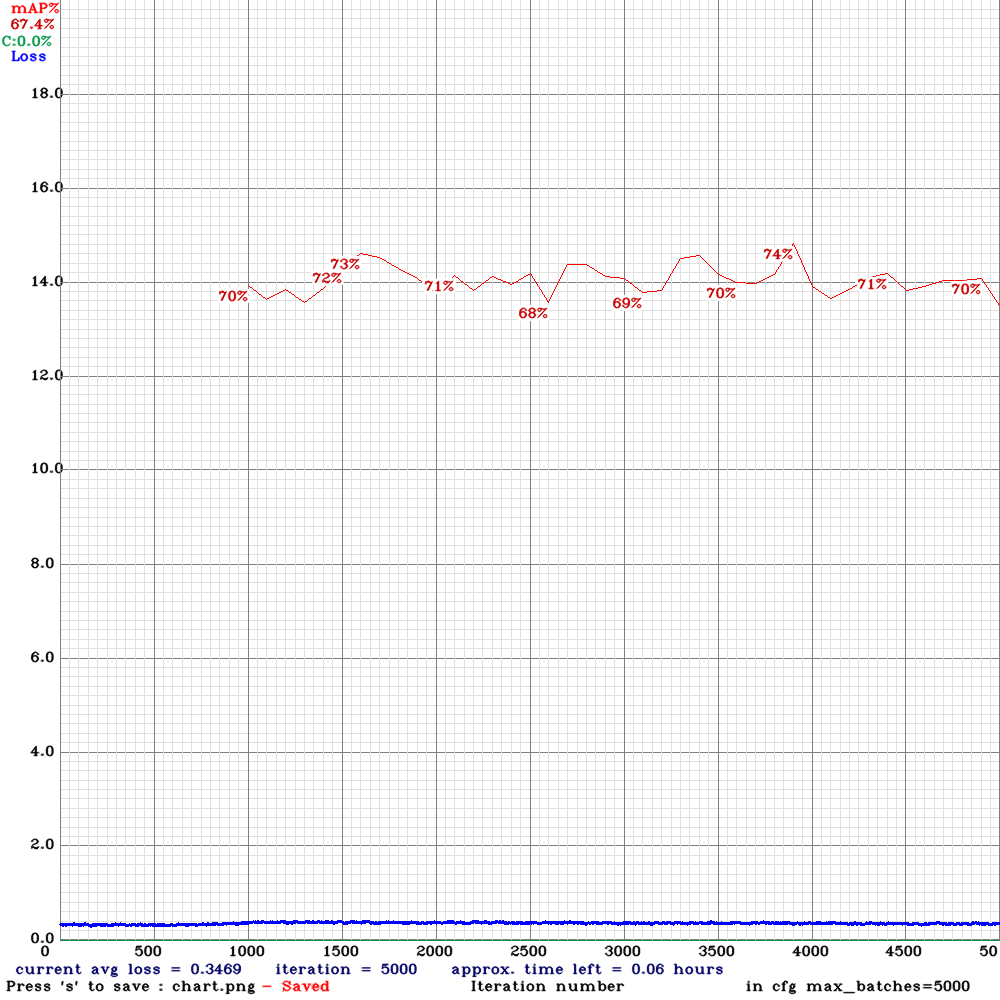
\includegraphics[width=5cm]{640-640-15000/chart.png}}}
	\caption \nolinebreak width=640, height=640 \\ red line: mAP
\end{figure}

		Như vậy, mô hình được lựa chọn là (width=544, height=544) sau 15000 max\_batch
	\item Cuối cùng, đánh giá mô hình được chọn trên tập test: 76.5\% mAP@0.5
\end{enumerate}



\subsection{Ứng dụng web}
\subsubsection{Giới thiệu}
Website cho phép người dùng tải lên một bức ảnh và lựa chọn sử dụng mô hình Yolov4-Tiny hay mô hình dự đoán động vật. 
Sau đó website sẽ trả về kết quả dự đoán: số lượng đối tượng, tên \& độ tự tin, ảnh kết quả với ô khoanh vị trí các đối tượng

\subsubsection{Chi tiết}
Website được viết bằng thư viện Flask trong python. Sau khi chạy script cài đặt, một web server sẽ được khởi tạo, cùng với đó là framework darknet và các file trọng số đại diện cho các mô hình. 
Ở đây ta có 2 file trọng số, đại diện cho 2 mô hình là Yolov4-Tiny và mô hình nhận diện động vật.

Khi người dùng truy cập vào trang web, tải ảnh lên, chọn loại mô hình và nhấn nút dự đoán, 
server sẽ tùy thuộc vào loại mô hình người dùng đã chọn mà dùng file trọng số tương ứng. Sau khi dự đoán xong, kết quả sẽ được hiển thị trên trang web. 
\subsection{Tài liệu tham khảo}
\begin{itemize}
	\item \url{https://github.com/AlexeyAB/darknet}
	\item \url{https://www.pyimagesearch.com/2017/12/04/how-to-create-a-deep-learning-dataset-using-google-images/}
\end{itemize}
\end{document}


